\chapter{System Design}
\label{system_design}
%intro maa fikses litt paa
This chapter presents our proposal for how a secure and restricted ad hoc network could be accomplished. It will cover which mechanisms described in Section \ref{system_authentication} we combine to ensure a secure and restricted ad hoc network and how they must be tailored to handle the special issues these kinds of networks introduce. The chapter then goes into details about how challenges regarding Public Key Infrastructures (PKI) and Certificate Authority (CA) hierarchies can be circumvented. Finally it gives the reader a technical description of how the BATMAN routing protocol should be modified and extended to handle the authentication.

\section{Design Overview} \label{design_overview}
Entities included in our system are much based on the ones described in Chapter \ref{background} and here we briefly describe the main roles of the entities and terminology used in our solution:

\begin{itemize}
\item \textbf{Service Proxy (SP)} is responsible for tasks similar to that of a CA or a node with an end entity certificate (EEC) as explained in Section \ref{system_authentication}. The SP is in possession of a Long-Lived Public Key Certificates (LLPKC) and has the ability to verify other LLPKCs belonging to nodes entering the network that the SP is managing. It is also allowed to sign Proxy Certificates which will be issued to nodes after they have been through an authentication process with the SP.

\item \textbf{Proxy Certificate (PC)} indicates a proxy certificate as described in Section \ref{background_pc} and more thoroughly in \cite{tuecke2004rfc3820}. In our system the term PC indicates a proxy certificate generated by a node that has not been signed yet. Depending on which entity that ends up signing the certificate, it will be named PC0, PC1 or PC2 as explained below.

\item \textbf{Proxy Certificate 0 (PC0)} is a proxy certificate belonging to a SP and is self-signed by the SPs LLPKC. This PC will have the certificate depth of 0 thus we refer to it as a PC0.

\item \textbf{Proxy Certificate 1 (PC1)} is a PC that can only be signed by a SP. The certificate is only signed if the node has as valid LLPKC. A node in possession of a PC1 is fully trusted node in the network managed by the SP who signed the certificate. It is not allowed to verify other LLPKC, but is delegated the right to sign PC2s which is explained next.

\item \textbf{Proxy Certificate 2 (PC2)} works in the same way as PC1 but with limited rights in the network. The restrictions put on the certificate are explained later in \ref{system_certificates}. The PC2 is either signed by a node in possession of a PC1 or the SP itself.

\item \textbf{Authentication List (AL)} is a list containing the necessary information about all the authorized nodes in a network. All nodes have a local AL which they use to decide whether they will process Originator Messages (OGM) received by neighbors. Their local lists are updated by an AL which is periodically broadcasted to all the nodes in the network by the SP. More details about this list is explained in Section \ref{al}.
\end{itemize}

\noindent
In our system, the OGMs sent by the BATMAN protocol have been modified to accommodate for additional information which will be used for authentication in the network. The authentication information is appended to an OGM by an Authentication Module (AM). For further referencing, we divide OGMs sent by a node in two types:
\begin{itemize}
\item \textbf{Plain OGM} refers to a regular OGM that does not contain any additional information added by the AM. This indicates that the OGM is sent from a node that does not belong to any network yet.

\item \textbf{OGM} indicates that the OGM was broadcasted by a node that has been authenticated somewhere and is thus part of some network.
\end{itemize}

\noindent
More about the format of the modified OGM and the AM is explained in Section \ref{am}.
\\\\
The essential idea of the system design explained in this chapter is that the nodes participating in a restricted network will only process routing updates from authorized nodes which have valid proxy certificates and are listed in their local Authentication List (AL). The example described in the next section illustrates the basic functionality of our system. 
\\\\
%Fix
The following sections explain more thoroughly the details about the how the authentication is done, gives a technical description of the modified BATMAN protocol and certificates used, and finally a discussion of the solutions challenges and limitations.

\subsection{Simple Example} \label{simple_example}
This example can be divided into three parts that show different important aspects of our solution.
\\\\
\textbf{Part I} Let us consider a very simple example where we have one SP present and one unauthenticated node A, both with empty ALs. The SP and node A will periodically broadcast OGMs as usual as part of the BATMAN protocol. Node A will broadcast plain OGMs as it is not part of any network yet. Upon reception of the plain OGMs from node A, the SP will engage in a handshake with A where node A is eventually issued a PC2 that is signed by the SP. % During this process the SP will also generate a self-signed PC0 if it does not have one already
\\\\
This is the general course of events for every node that enters a network it is not already authenticated in and is within transmitting range of SP. Figure \ref{fig:first_auth_msc} is a message sequence chart (MSC) illustrating the messages exchanged in this scenario.
\\
\begin{figure}[ht]
	\centering
		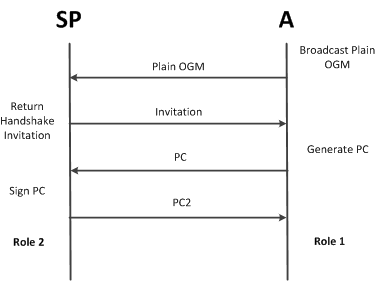
\includegraphics{images/first_auth_msc.png}
	\caption{Initial handshake between the SP and Node A, which results in Node A getting a PC2.}
	\label{fig:first_auth_msc}
\end{figure}

\noindent
\textbf{Part II} After node A has received its new certificate, it will now start using the additional authentication fields in its OGMs to show that it is in possession of an PC2. %Since the SP has signed the certificate, it is now able to verify the OGMs received from node A. However, since node A only has a PC2 in this network, it has limited rights on what it is allowed to do in the network and other nodes that might be part of the network, will process OGMs sent from this node differently. This is explained further in Section \ref{system_certificates}
\\\\
When the SP receives the new OGMs from node A, it knows that A might be able to be upgraded with a PC1. So upon the reception of an OGM from A, the SP will again invite to a new handshake which is somewhat similar to the one described above, only here the nodes also validate each others LLPKC. The authentication process is finalized when node A is issued a PC1 signed by the SP and becomes a fully trusted node in the network.
\\\\
Figure \ref{fig:first_env} shows how the network is established and how the nodes ALs and certificates change during the different steps in the authentication process.

\begin{figure}[ht]
	\centering
		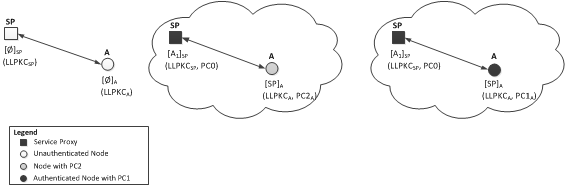
\includegraphics{images/simple_first_env_tot.png}
	\caption{Illustrates stepwise how a network is established between a node A and SP, both with valid LLPKC}
	\label{fig:first_env}
\end{figure}

\noindent
If a node possessing a PC2 and a LLPKC is a direct neighbor with the SP, the following course of events will be as depicted in  Figure \ref{fig:first_env}. This is of course only true if the SP can recognize and verify the PC2 and the LLPKC.
\\\\
\textbf{Part III} If however an unauthenticated node is not within transmitting range of the SP, the plain OGMs might still reach some of the other nodes in the network. To be able to authenticate this new node, we use the fact that nodes in possession of a PC1 are allowed to sign PC2 certificates. To show how a new node can join a network without being in direct contact with the SP, let us imagine the following scenario: Node B now wants to join the restricted network established by the SP and node A shown in Figure \ref{fig:simple_sec_env_1} and it is only able reach node A with its OGMs.
\\
\begin{figure}[ht]
	\centering
		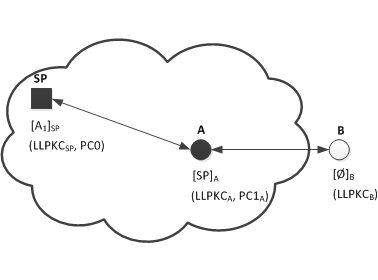
\includegraphics{images/simple_sec_env_1.png}
	\caption{The figure shows a new unauthenticated node B entering a restricted network with node A an SP. Also depicted is a simplified AL and certificates.}
	\label{fig:simple_sec_env_1}
\end{figure}

\noindent
Because node A has a PC1 it is able to sign and issue a PC2 to B such that it is now untrusted member of the network. The OGMs sent from node B will eventually reach the SP through A and the SP is also able to verify the OGMs because it has a PC2 signed by As PC1. The SP will then recognize that since node B only has PC2 it may be qualified to be upgraded with a PC1. Thus the SP will initiate a handshake similar to the one explained in Part II. If it has a valid LLPKC, node B will be issued a PC1 and also become a fully trusted member of the network.

\section{Authentication} \label{system_authentication}
This section presents in detail how the authentication process is done when exchanging and verifying certificates between nodes. It also goes into detail on what is actually sent in the messages during the two different handshakes mentioned in the previous section, which have been called Initial and Authentication Handshake respectively.

\subsection{Initial Handshake}
The first handshake that an unauthenticated node is involved in is between the new node and the SP as depicted in Part I in the example above. This handshake is called an initial handshake.
\\\\
During this initial handshake, the unauthenticated node will generate a public key pair and a corresponding PC. It sends this PC to the authenticated node which will in turn sign it with its private key from PC1. The PC then returned is thus what we call a PC2. The process is the same if the signing node is the SP, the only difference is that the private key from its PC0 is used to sign the certificate, and the new node will still get a PC2. When this step is complete the new node will be able to use his PC2 to identify itself as a node with limited rights in the network, and also use it for encryption in a new handshake.

%This handshake can also happen between the new node and an authenticated node in the network as shown in Part III.

\subsubsection*{Message Exchange in Initial Handshake}
Here we show more detailed what information the Authentication Module (AM) exchanges during a initial handshake between a new unauthenticated node A and a regular authenticated node B. Public and private keys are denoted as PU and PR respectively, and they belong to the certificate being used by the sender node. A nonce is represented by N, encryption E and Proxy certificates are denoted PC. The handshake is triggered by B receiving a plain OGM from A and continues as follows:

\begin{enumerate}[I]
\item $B \rightarrow A: N_{B} $
\item $A \rightarrow B: PC_{A}\{PU_{A}\} \: || \: E_{PR_{A}}(N_{B}) $
\item $B \rightarrow A: PC2_{A}\{PU_{A}, \: E_{PR_{B}}(Hash[PC_{A}])\} $ 
\end{enumerate}

\noindent
The nonce value sent in message I is the invitation to the initial handshake. Node A responds with a self-generated PC and proves it owns the certificate by using the corresponding private key to encrypt the nonce value. Node B checks the nonce value by decrypting the message and comparing it to the sent nonce with the public key extracted from the PC, $D_{PU_{A}}(E_{PR_{A}}(N_{B})) = N_{B}$. Then node B signs the certificate, effectively making it a PC2 and sends it back to node A. It is important to notice that B never reveals its PC1 or public key.
\\\\
What is shown in this list is a minimum requirement of what should be put in the messages sent. Certificates such as the PC should however contain much more information than just e.g. the public key. However, it is not necessary to include this information here since it has no impact on how the handshake is performed, but it will be discussed in Section \ref{system_certificates}.

\subsection{Authentication Handshake}\label{authentication_handshake}
If the SP discovers a new node with a PC2 in its network, it will invite the node to what we called an authentication handshake. This handshake is shown in both Part II and III in the simple example above. The goal of the handshake is to establish full trust between the nodes with a mutual authentication where they verify each others' LLPKC. In this handshake, the SP will make use of the encryption channel established in the initial handshake to protect and reduce the exposure of important information, such as the LLPKC.

\subsubsection*{Message Exchange in Authentication Handshake}
The message exchange in this section is denoted in the same manner as previously. The only difference is that we also handle LLPKC certificates.
\\\\
The first three messages shown below will always take place during the authentication handshake. The important thing that happens here is that node A sends its LLPKC to the SP. The authentication handshake is initiated when the SP receives an OGM that indicates that it has a PC2 and no PC1. This is shown in message I where a digital signature of the OGM is appended. This we will come back to later.

\begin{enumerate}[I]
\item $A \rightarrow SP: OGM_{A} \: || \: E_{PR_{PC2_{A}}}(Hash[OGM_{A}])$
\item $SP \rightarrow A: E_{PU_{PC2_{A}}}(N_{SP})$
\item $A \rightarrow SP: E_{PR_{PC2_{A}}}(LLPKC_{A}, \: E_{PR_{LLPKC_{A}}}(N_{SP}, \: N_{A}))$
\end{enumerate}

\noindent
The next step of the handshake depends on whether the SP finds the LLPKC from node A valid. If it does so, the SP will return its own LLPKC back to A for mutual authentication. The observant reader will notice that the public keys for the LLPKC and PC0 of SP is never revealed to an untrusted node.

\begin{enumerate}[I]
\setcounter{enumi}{3}
\item $SP \rightarrow A: E_{PU_{LLPKC_{A}}}(LLPKC_{SP}, \: E_{PR_{LLPKC_{SP}}}(N_{A}, \: N_{SP}))$
\end{enumerate}

\noindent
If node A can verify the LLPKC of SP, the handshake is continued. Otherwise it will be aborted at this point. The rest of the handshake is similar to the initial handshake, except that it will be done in privacy with help of the keys from the LLPKCs.
\\\\
The last messages below show that A generates a new PC which is signed by the SP making it a PC1. The last message of the handshake provides node A with its own PC1 and the PC0 of the SP such that it can verify routing messages from the SP.

\begin{enumerate}[I]
\setcounter{enumi}{4}
\item $A \rightarrow SP: E_{PU_{LLPKC_{SP}}}(PC_{A}\{PU_{PC_{A}}\})$
\item $SP \rightarrow A: E_{PU_{LLPKC_{A}}}(E_{PR_{LLPKC_{SP}}}(PC1_{A}\{PU_{PC1_{A}}, \: E_{PR_{PC0_{SP}}}(Hash[PC_{A}])\}, \: PC0_{SP}))$
\end{enumerate}


\section{Authentication Module} \label{am}
This section show how the original BATMAN protocol should be modified to incorporate our authentication scheme. Here we introduce the Authentication Module (AM), explain how it changes the OGMs and the general BATMAN routing flow. The AM is responsible for handling three things: OGM signatures, handshake messages, and broadcasting of Authentication Lists which will be described later. 

\subsection{OGM Signature} \label{ogm_signature}
The Originator Message (OGM) as described in the original BATMAN protocol, has been modified such that it includes the number and lengths of the fields appended by the Authentication Module. These fields are used to contain signatures that a node uses to authenticate itself when sending or rebroadcasting an OGM. A node should be able to append several signatures as it can be a member of several networks using different PCs with different key pairs, e.g. PC1 in one network and PC2 in a different one.
\\\\
The signature is a encrypted hash made from all static fields in the OGM, i.e. version number, sequence number and the originator address, in addition to the sequence number.
\\\\
Hashing and signing an OGM every time it is sent between nodes would introduce a high computational cost and be time consuming for the resource limited nodes. Additionally, it would add a lot of network load, and it is difficult to predict how well the network would handle all the extra routing traffic load. A suggestion would then be that the signature should only be generated periodically. I.e. if we chose a time interval of say 60-120 seconds, the signature will only changed and sent for every 60-120 seconds that has passed. In between the time interval, only a small number of bits constituting the most significant bits of the signature will be appended to the OGM.
\\\\
When a node receives an OGM from its neighbor for the first time, or when the node has produced a new signature, it checks the signature by calculating the hash of the OGM and comparing it to the decrypted signature appended to the OGM. If they are the same, the fraction of most significant bits is stored alongside the neighbor node in the local AL.
\\\\
For the next OGM it receives, it will check its local AL for the most significant bits of the signed hash that belongs to this node and compare it to the signature fraction appended to the OGM. If the signature fractions are equal, the node is still authenticated and the OGM will be processed. If not verified, the OGM will be dropped. The hash values stored in the AL must be updated ever time a node generates a new signature for its OGMs.
\\\\
Because of the likelihood of packet loss in ad hoc networks, the receiving neighbor node does not require to see a new signature from the originator at the same rate as the originator is sending them. It only needs to see a new signature (and new subsequent fractions) within a reasonable window period, e.g. 3-5 times the signature update frequency. However, if that window passes and no new signature is received, it will start dropping the OGMs and remove the node as a direct neighbor. 
\\\\
The interval for when a node should update its signature and send OGMs containing signatures, is a trade-off between security in the likelihood of replay attacks i.e. how many replayed OGMs is needed to change the routing topology significantly, and of computational cost.
%\\\\
%If a node receives an OGM from its neighbor and does not recognize the signature fraction, it receives an old fraction outside the time frame, or it receives a full signature it cannot verify - it will drop the OGM. This will lead to new direct neighbors always dropping the OGM in the beginning, because you will only see and store signatures from your direct neighbor.

\subsection{Handshake Messages} \label{am_handshake}
The Authentication Module has the responsibility of the handshakes as explained in Section \ref{system_authentication}. I.e. it reacts on plain OGMs, creates nonces, has the cryptographic functions and so on. When the module starts or reacts to a handshake, it does so in parallel of normal of the BATMAN operations. Handshake messages are sent using plain UDP datagrams, completely separated from OGMs. The UDP datagrams are also directly addressed to the recipient is possible, and not broadcasted to every node in the network.

\subsection{Authentication List Broadcast}
As with handshakes, the authentication lists are completely handled by the Authentication Module. The AM maintains the local copy and takes care of broadcasting the AL in UDP datagrams. %These ALs will most likely be too large to fit in one datagram, and they will therefore be split up into several datagrams. We still will not add any reliable delivery method, because of the way broadcasting in the network works we expect every node to get the complete AL eventually, even if one datagram is lost.

\section{Authentication List} \label{al}
The authentication list is used for continuous node authentication during routing. The SP is responsible for broadcasting this list periodically such that every node in the network will have an updated local list over nodes that have been authenticated in the network. The AL is a table where every node is represented with a row which should at least contain the following elements:

\begin{itemize}
\item \textbf{Node ID} The unique idenity from the proxy certificate which is an unique identifier of the node owning the certificate. The ID ties the correct node to the right signature.
\item \textbf{Originator address} IP address of the authenticated node.
\item \textbf{Public key} Public key of the corresponding node.
\item \textbf{Role} Indicates whether the originator has a PC0, PC1 or PC2 certificate. This will affect how an OGM is processed after its sender has been authenticated.
\item \textbf{Validity Period} The lifetime of the nodes PC. 
\item \textbf{Digital Signature Fraction} The fraction of the most significant bits of the last verified signature.
\item \textbf{Last Signature Received} Timestamp of the last received signature.
\end{itemize}

\noindent
Upon broadcasting the AL, the SP will encrypt the list with its private key from its LLPKC guaranteeing its confidentiality and integrity as well as signing it afterwards with its PC0 for authenticity. Every node in the network has an explicit or implicit trust of the SP to sign and verify new nodes; therefore every node will trust the content of this list even if it is received through another node in the network.
\\\\
We differ between two types of Authentication Lists - one which is a complete list of all the authenticated nodes in the network, and one which is only a single entry update containing new nodes that have been issued a PC2 from a trusted node, or PC1 from a SP.
\\\\
When a trusted node has signed a new nodes PC2, it needs to make the other nodes aware of this node thus needs to be able to update the other nodes AL with this node. The trusted node then makes use of the single row AL, and signs the AL update with its PC1. It does not however, encrypt the message as the SP would do with the full list. Encryption of this update is not necessary, as the information about a new node with PC2 is not regarded as confidential. Neighboring nodes will add this new node to their local ALs and rebroadcast the list until every node in the network has it. When every node has received the AL update, they will be able to forward the new nodes OGMs, which will then finally reach the SP and trigger the authentication handshake.
\\\\
A node with PC2 is not able to read the AL that is broadcasted from the SP as it is not in possession of the public key of SPs LLPKC that can decrypt the list. This way, we still protect the public keys of the SPs and trusted nodes.

\section{Certificates} \label{system_certificates}
The certificates used in our system design are Long-Lived Public Key Certificates (LLPKC) and different types of Proxy Certificates (PC). The reasoning for why we have chosen to use these certificates is explained in this section.

\subsection{Long-Lived Public Key Certificates}
These certificates are used for identity authentication which may, if recognized, give the owner full access rights to the network. It is also in these certificates stated explicitly whether the owner can assume the SP role. These certificates will typically be issued before arriving at the scene of the BATMAN network. The LLPKC may be regular X.509 certificates as explained in Section \ref{LLPKC}.

\subsection{Proxy Certificates}
One of the benefits of choosing proxy certificates in our system is their ability to define nodes rights in the network in their assigned certificates. By utilizing the Restricted Proxy Certificate (RPC) explained in Section \ref{background_pc} these rights are decided by the node who signs the certificate and are be specified in an appropriate language. A PC can be created with any desired lifetime and will in our case typically be given a lifetime that is significantly shorter than the LLPKC. This fits well with the highly mobile nodes that are assumed to be in these kinds of networks and the environments in which they are to be used.
\\\\
As mentioned in the design overview in section \ref{design_overview}, we differ between three types of proxy certificates: PC0, PC1, and PC2. PC0 is the certificate with the highest rights and is self-signed by the SPs own LLPKC. It is able to establish a proper network and to verify and sign new PC1s to authorized and trusted nodes. In addition the node in possession of a PC0 is also allowed to broadcast the full Authentication List.
\\\\
PC1 on the other hand is not allowed to sign new PC1s, but can sign PC2. This is such that node can be able to join the network without being in direct contact with the SP. A PC1 is also allowed to broadcast a AL containing a new PC2 that it has just allowed into the network. This must be possible because the OGM then sent from the node with PC2 must be allowed to be forwarded in the network as well such that it will eventually reach the SP. This way, it can be authenticated properly if it has a valid LLPKC, and the network is also able to grow without being too dependent on the SP. It also relaxes some of the load on the SP.
\\\\
A node with a PC2 has the most restricted role in a network. Trusted nodes in the network will only accept the PC2s own OGMs, not if it rebroadcasts any others OGMs. Thus the network will be aware of the node with the PC2, but not any other networks the node might be connected to. %With this restriction, the network is also protected from route-spoofing attacks of the new node, as it cannot change routing information.
\\\\
As everyone will be aware of the node, the SP is able to do a new authentication handshake and check if it can be upgraded with a PC1. But until it does, it will have limited influence on the existing network and the routing done within it.
\\\\
A specific cryptographic scheme for the proxy certificates has not been decided yet, but Elliptic Curve Cryptography looks promising given its short keys. As the SPs have to periodically broadcast the public keys in the ALs, keeping the size to a minimum is of importance.


\section{Service Proxy Presence}
This section explains what happens if there are no service proxy (SP) present when establishing a network. It also describes what happens when a SP enters a network which is established by only regular nodes.
\\\\
Two nodes discover each other in such a situation by broadcasting Plain OGMs as normal. They may both be in possession of LLPKCs, but there is however no SP present that can verify them. Even though there is no SP in the network, it is preferred that one of the nodes should become a master node which would have similar but limited rights as the SP.
\\\\
How this role is assigned can be done in several ways. One suggestion is mentioned in an essay that can be found in Appendix \ref{essay}. However, to keep things simple in our implementation, an easy way to implement this would be to let the node with the lowest link layer address assume the master role.
\\\\
The master node could generate a self-signed certificate, PC0 for which it can use to sign new PC1s to nodes entering the network. It is up to the master nodes whether it will allow every node that it discovers access to the network, or if they must have LLPKCs signed by the same CA as itself. We leave this choice to the users of the protocol because this depends on the setting in which the protocol is used.
\\\\
After such a network has been established, a SP may join at a later point in time. When the SP is in close proximity of the network, it will immediately start receiving the OGMs that are broadcasted in the network. As it is not able to recognize and verify the OGMs sent, it will automatically initiate a handshake with these nodes, issuing PC1 or PC2 depending on what kind of certificates they have. This way the SP will effectively be able to take over the management of the network after some convergence time. 
\\\\
It is important to consider such scenarios as this, because it might not always be the case that a node that can act as a SP is present at a location. It is then important that the nodes are still able to configure a network between them 

\section{Network Merging}
When two networks are within the same vicinity they may want to be able to merge such that they are able to co-operate or to use each other as a resource. Given the scenarios described in Chapter \ref{scenario_requirements} the reason for merging becomes even clearer. This section will discuss how a limited merging will happen automatically as a consequence of how the protocol/system works now and how it can be extended to make a more complete merging.

\subsection{Limited Merging}
A node which is a trusted member in one network, i.e. has a PC1 here, is also able at the same time to have a PC2 belonging to another network.
\\\\
The node will continue to broadcast its OGMs as usual, but now appended with signatures made with both proxy certificates. However, it will only rebroadcast OGMs from the network where it is fully trusted and not in the one where it only has a PC2, as defined in Section \ref{system_certificates}. The node will also only use the PC1 connected to the specific network in which it sends the rebroadcast. I.e. it will only add the PC1 from the first network in its rebroadcasts of OGMs from that network, and it will discard OGMs from the new network where it only has a PC2.

\begin{figure}[ht]
	\centering
		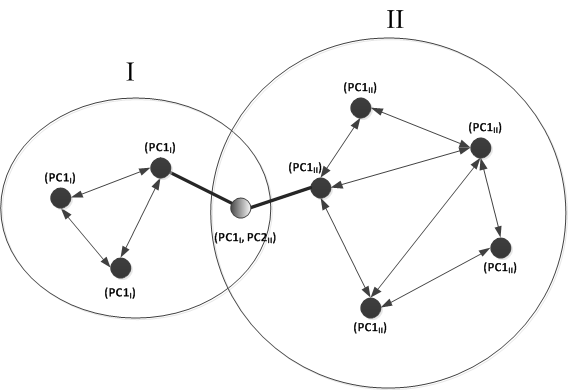
\includegraphics{images/limited_merging.png}
	\caption{Limited merging between two networks, I and II, with one node in possession of PC1$_{I}$ and PC2$_{II}$ acting as gateway between the networks.}
	\label{fig:limited_merging}
\end{figure}

\noindent
\\\\
In order for this limited merging to be of any value for the networks, the node needs to be able to broadcast the network prefix of each network, becoming a gateway node, to each other so that nodes in both networks can communicate with each other through the gateway node. It is important to notice that nodes in one network will not get routing updates from the other network, and they will not learn about each other before another entity takes care of this information. For instance, a special node could get a PC1 from every network on site using e.g. out-of-band authentication and then become a DNS server for the site. We wont go into more detail on this because that is not part of our scope, but can be interesting to note.
\\\\
This functionality may be very beneficial for some parties, but too insecure for others - therefore we note that this functionality needs to be optional for the users. For example, in a large emergency situation a few actors like civilian paramedics and The Red Cross personnel might want this functionality, but the military might want to opt out to protect their secure network.


\subsection{Full Merging}\label{full_merging}
The limited merged network explained above does not scale very well, and should only be used temporarily until the networks can be fully merged. For the networks to be fully merged there needs to be some trust established between the different service proxies managing the networks. 
\\\\
If the SPs are able to verify each others as trusted SPs based each others LLPKC, then each SP can sign each other a PC0 for each others network. This way, they both become SPs in a large fully merged network. If they are not able to reach each other, or not verify each others LLPKC they should be able to use an out-of-band authentication. As before, we will not go further into how this is done, but it is worth mentioning.
\\\\
After the SPs have signed each others PC0, they will send their ALs to each other in order to make a full AL for the whole fully merged network. After this point, all nodes in all merged networks will be able to verify each other and from the point of view of the regular nodes the network merging is complete.
\\\\
The SPs however, needs to decide upon a master SP which will take care of new unauthenticated nodes and broadcasting the full AL. The choice might be different based on the requirements of the users. I.e. it might be done in a arbitrarily fashion, or it might be determined out-of-band based on some real-world characteristics.


\section{Assumptions and Limitations}
Some assumptions have been made to make our system design possible. These are explained here in this section as well as potential limitations these assumptions may introduce.

\subsection{Pre-Configured Long-Lived Public Key Certificates}
In our system design we have assumed that before a node can be issued a PC1 and become a fully trusted node, it is obligated to present a valid LLPKC to the SP managing that network. This means that all nodes must be given a LLPKC signed by a CA at some point to be able to connect to a restricted network. This certificate could either be manually pre-configured or perhaps given to the node out-of-band sometime. 
\\\\
However, even though a node is in possession of a LLPKC it might still not be recognized by the current SP. In that case the node will only be issued a PC2 until it eventually gets a certificate which is valid. This can be given to the node through some out-of-band authorization which leads to the SP signing the node a new LLPKC, and revoking it when the scenario is over. Thus the node would get full access to the network for a limited time.
\\\\
If a node is not in possession of any LLPKC at all, it is still able to be part of the network with the help of a PC2. This way we assure that the network is aware of nodes that may potentially be important and should consider being issued a PC1 or LLPKC trough the network or out-of-band.
\\\\
However, this is something that could be up to the SP to decide. If it finds it necessary to establish a network without validating LLPKC, it could issue PC1 to all nodes who want to participate in a network. The SP is then creating a network that is restricted in the sense that only nodes in the network are able to communicate with each other and the only way to get an certificate would be through the SP.
\\\\
The reason for why we use LLPKC in our system design is in order to do a full authentication of nodes. That is, with a LLPKC you are able to have a unique relation between an identity and its certificate. It is therefore a good way of providing a verification of an identity, while the proxy certificates are primarily used for verifying that the node in possession of it have access to the network, it can be indifferent of the real identity of the node given the settings of the SP.

\subsection{Service Proxies - Operational Command Centers}
The Service Proxy is a central entity which is in charge of the access control in a network. It is argued that central nodes are not preferred in ad hoc network as they violate the goal of a truly decentralized network. However, to be able to have a proper authentication scheme in our system, it is necessary to have some central nodes that can handle the access control to the network. These task of a central node can tied to the responsible operational center on the site, as described in Chapter \ref{scenario_requirements}.

\subsection{Valid LLPKCs}
During the authentication handshakes, the SP might not have access to the Internet and thus not able to get the latest copies of the Certificate Revocation Lists (CRL). This means that even though an SP is able to verify nodes LLPKC, it might have been marked as invalid/revoked in the CRL. We assume however that the SP will authenticate new nodes based on the knowledge it has at the moment of authentication, and rather check with the CRLs after an Internet gateway has been set up. %hvorfor er dette viktig? kommer ikke paa noe lurt aa skrive

\subsection{Multi-Layered Security}
Security is a multi-layered issue and we consider only routing done on the network-layer in our system design. We assume users of our protocols use proper transport- and application-layer security protocols. The proxy certificates used in our system is meant for routing-security, and we assume they are not used for security on the layers above. We therefore assume our PCs and LLPKCs are used for hardware authentication, not user authentication which would be handled upper layers.

\subsection{IP Allocation}
When a new node is discovered, it would probably have a link-local IP address which in turn requires that an address allocation scheme must be in place, e.g. DHCP. This responsibility would be natural to assign to the SP, but depending on the network configuration other nodes could also be in charge of this. In our scheme we do not however cover this setup, and we use static IP allocation in our implementation explained in Chapter \ref{implementation}.

\section{Security Considerations and Issues}
In this section we cover some of security considerations and issues that is worth mentioning. 

\subsection{Public Keys}
One of the security features of our system is that the public keys belonging to the PC0s, PC1s and the SPs LLPKCs are only public inside the network of fully trusted nodes. This enables us to use the private key of the PC1s belonging to trusted nodes and LLPKC to the SP to encrypt the authentication lists broadcasted thus the lists will only be readable for nodes inside the network. % as explained in Section \ref{al}.
\\\\
However, using the private key for signing and encrypting is not recommended as this might expose the key to potential cryptanalytic attacks. But for the SP it only uses the private key of its LLPKC to self-sign its own PC0, thus not exposing its key in such degree.

\subsection{Security Issues}
Being based on a wireless network, our system is vulnerable to security attacks that take advantage of this shared medium. Attacks such as Denial of Service (DoS), "man-in-the-middle" and jamming can severely paralyze and damage a communications network and can be very hard to avoid \cite{1625756}. Protecting our system against these kinds of attacks would be challenging. 

%man-in-the-middle attack eksempel?

